\documentclass[11pt]{article}
% Shared LaTeX preamble for Watchdog docs.
\usepackage[margin=1in]{geometry}
\usepackage[T1]{fontenc}
\usepackage{lmodern}
\usepackage{microtype}
\usepackage{graphicx}
\usepackage{xcolor}
\usepackage{hyperref}
\usepackage{booktabs}
\usepackage{longtable}
\usepackage{enumitem}
\usepackage{titlesec}

\hypersetup{
  colorlinks=true,
  linkcolor=blue,
  urlcolor=blue,
  citecolor=blue
}

\setlist[itemize]{noitemsep,topsep=2pt,leftmargin=1.2em}
\setlist[enumerate]{noitemsep,topsep=2pt,leftmargin=1.6em}

\titleformat{\section}{\Large\bfseries}{\thesection}{0.6em}{}
\titleformat{\subsection}{\large\bfseries}{\thesubsection}{0.6em}{}

\newcommand{\watchdog}{Watchdog}
\newcommand{\service}[1]{\texttt{#1}}
\newcommand{\apiendpoint}[1]{\texttt{#1}}

% Diagrams are rendered to ../diagrams/images (relative to docs/latex).
\graphicspath{{../diagrams/images/}}


\title{\watchdog{} --- Architecture Document}
\author{}
\date{March 20, 2026}

\begin{document}
\maketitle

\section{Purpose and Scope}
\watchdog{} is a service-oriented monitoring and incident triage platform.
It ingests logs/metrics, reduces noise, opens incident tickets, and enriches incidents with NLP-based classification.

\section{Current Codebase Snapshot}
This repository currently contains three services:
\begin{itemize}
  \item \service{watcher-service} (Go): ingestion + basic event normalization
  \item \service{core-service} (Spring Boot): ticket APIs + orchestration starter
  \item \service{nlp-service} (FastAPI): enrichment API (heuristic stub)
\end{itemize}

\section{System Context}
\begin{figure}[h]
  \centering
  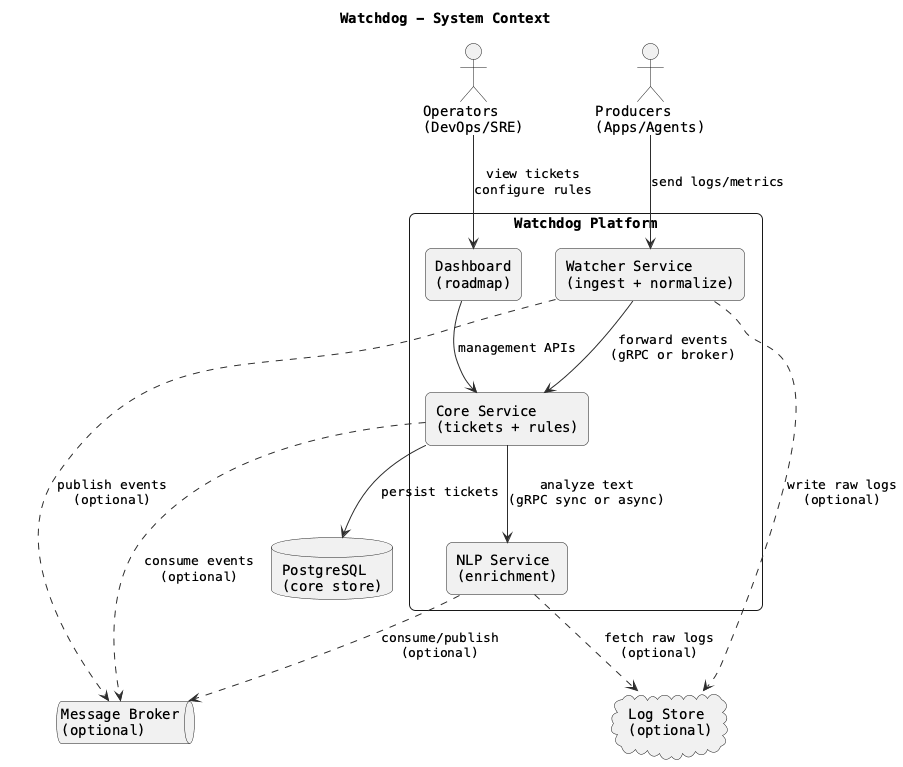
\includegraphics[width=\linewidth]{system-context.png}
  \caption{System context}
\end{figure}

\section{Features (Simple English)}

This section lists what \watchdog{} does (and what it is planned to do) using simple, non-jargon language.

\subsection{Ingestion and Normalization}
\begin{itemize}
  \item Accept logs and metrics over HTTP from external producers.
  \item Validate the incoming payload (required fields, supported kinds, size limits).
  \item Normalize the event shape so downstream services see consistent fields.
  \item Classify incoming data as either a \emph{log} (reactive) or a \emph{metric} (proactive).
  \item Provide health endpoints so operators can verify the service is up.
\end{itemize}

\subsection{Incident (Ticket) Management}
\begin{itemize}
  \item Create an incident ticket when a critical condition is detected.
  \item Track ticket status through a small lifecycle: \texttt{OPEN} $\rightarrow$ \texttt{INVESTIGATING} $\rightarrow$ \texttt{RESOLVED}.
  \item List and fetch tickets so an operator can see what is happening.
  \item Allow an operator to manually update a ticket (status and notes/comments).
\end{itemize}

\subsection{Rules and Proactive Alerts}
\begin{itemize}
  \item Evaluate metrics against thresholds (for example, ``error rate too high'').
  \item Reduce noise by suppressing duplicates and ignoring low-signal events (roadmap).
  \item Support backpressure so bursts of data do not overwhelm the system (roadmap).
\end{itemize}

\subsection{NLP Enrichment (Intelligence Layer)}
\begin{itemize}
  \item Analyze log text and return: category (example: database), severity, confidence score, and extracted keywords/entities.
  \item Support a basic heuristic mode today and model-backed inference later.
\end{itemize}

\subsection{Security and Access Control}
\begin{itemize}
  \item Protect management APIs with authentication (JWT in the current starter; real JWT validation and RBAC are planned).
  \item Keep health checks unauthenticated for infrastructure probes.
  \item Plan for secure service-to-service calls (mTLS / service identity) once traffic patterns stabilize.
\end{itemize}

\subsection{Observability and Operations}
\begin{itemize}
  \item Emit logs and basic health endpoints from each service.
  \item Plan for metrics endpoints compatible with Prometheus and dashboards in Grafana.
  \item Plan for tracing and correlation IDs across services.
\end{itemize}

\subsection{User Interface (Roadmap)}
\begin{itemize}
  \item Provide a real-time dashboard to view active tickets and recent events (roadmap).
  \item Provide admin screens for user management and configuration (roadmap).
\end{itemize}


\section{Architecture Prototypes (SOA/Microservices)}

The goal of this section is to propose multiple \emph{simple} but \emph{detailed} candidate architectures.
We will later compare trade-offs and choose one.

\subsection{Shared Principles (All Prototypes)}
\begin{itemize}
  \item Clear service boundaries: ingestion (\service{watcher-service}), orchestration (\service{core-service}), enrichment (\service{nlp-service}).
  \item A stable contract for events and APIs (schemas under \texttt{contracts/}).
  \item Database-per-service (start with PostgreSQL for \service{core-service}; keep others stateless where possible).
  \item Idempotency and correlation IDs for safe retries.
  \item Health endpoints on every service.
\end{itemize}

\subsection{Prototype A: Direct Orchestration (No Broker)}
\textbf{Intent:} minimize infrastructure and complexity; good for early MVP.

\begin{itemize}
  \item External producers send events to \service{watcher-service}.
  \item \service{watcher-service} validates and normalizes events, then calls \service{core-service} via gRPC.
  \item \service{core-service} persists tickets and calls \service{nlp-service} via gRPC when log text needs enrichment.
  \item All flows are request/response; retries use idempotency keys.
\end{itemize}

\textbf{Key contracts (suggested):}
\begin{itemize}
  \item Public ingestion: \apiendpoint{POST /api/v1/ingest} to \service{watcher-service}.
  \item Internal event handoff (gRPC): \texttt{watchdog.core.v1.EventIngestor/SubmitEvent}.
  \item Internal enrichment (gRPC): \texttt{watchdog.nlp.v1.Analyzer/Analyze}.
\end{itemize}

\textbf{Failure and retry behavior:}
\begin{itemize}
  \item If \service{core-service} is slow/unavailable, \service{watcher-service} must apply timeouts and safe retries.
  \item Use \texttt{event\_id} as an idempotency key so \service{core-service} can safely ignore duplicates.
  \item If \service{nlp-service} fails, \service{core-service} should still create the ticket and mark enrichment as pending.
\end{itemize}

\begin{figure}[h]
  \centering
  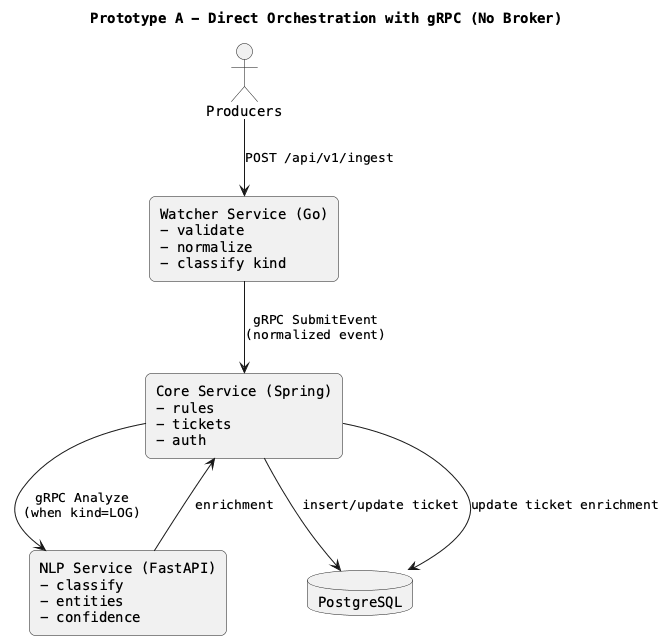
\includegraphics[width=\linewidth]{prototype-a-direct-rest.png}
  \caption{Prototype A: Direct REST orchestration}
\end{figure}

\subsection{Prototype B: Event-Driven With Message Broker (Recommended Direction)}
\textbf{Intent:} decouple ingestion from orchestration; enable buffering and smoother scaling.

\begin{itemize}
  \item \service{watcher-service} publishes normalized events to a broker (RabbitMQ/Kafka).
  \item \service{core-service} consumes events and decides: open/update tickets, or ignore.
  \item \service{nlp-service} can be invoked either synchronously by \service{core-service} via gRPC or asynchronously by subscribing to log events.
  \item Use a dead-letter queue (DLQ) and replay tooling to handle poison messages.
\end{itemize}

\textbf{Suggested topics/queues:}
\begin{itemize}
  \item \texttt{watchdog.normalized-events} (all events) or split by kind: \texttt{watchdog.logs}, \texttt{watchdog.metrics}
  \item \texttt{watchdog.enrichment-events} (enrichment results)
  \item \texttt{watchdog.dlq} (dead letters after max retries)
\end{itemize}

\textbf{Processing model:}
\begin{itemize}
  \item At-least-once delivery: consumers must be idempotent (dedupe by \texttt{event\_id}).
  \item Backpressure is handled by the broker (queue depth) rather than by making producers wait.
  \item A ``poison message'' lands in DLQ with enough metadata to replay after fixing the root cause.
\end{itemize}

\begin{figure}[h]
  \centering
  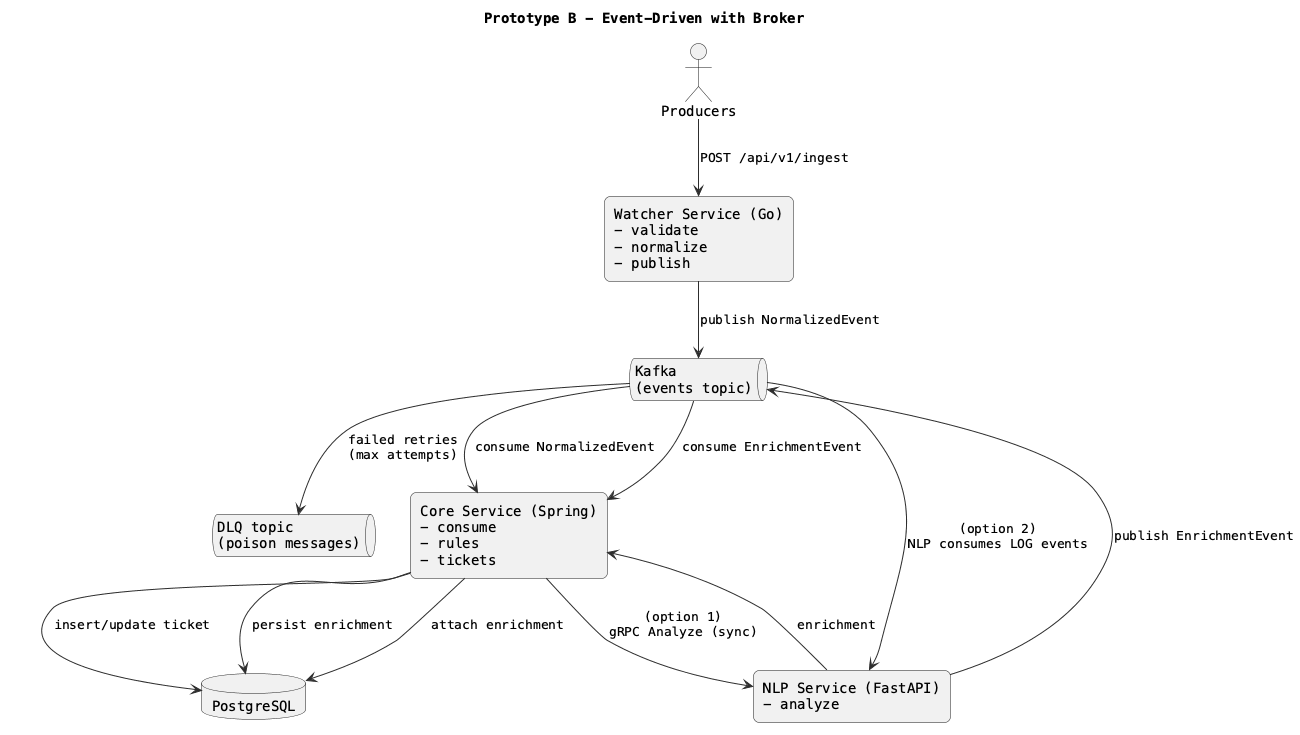
\includegraphics[width=\linewidth]{prototype-b-event-driven.png}
  \caption{Prototype B: Event-driven ingestion and processing}
\end{figure}

\subsection{Prototype C: Pipeline With Log Store + Async Enrichment}
\textbf{Intent:} separate large/raw log payload storage from ticket decisions; keep event bus lean.

\begin{itemize}
  \item \service{watcher-service} writes raw logs to a log store (OpenSearch/ELK/Object Storage) and publishes a small ``pointer event'' to the broker.
  \item \service{core-service} consumes pointer events and applies rules to open/update tickets.
  \item \service{nlp-service} consumes pointer events, fetches full text from the log store, computes enrichment, and writes results back.
  \item \service{core-service} attaches enrichment to tickets asynchronously (eventual consistency).
\end{itemize}

\textbf{Pointer event (example fields):}
\begin{itemize}
  \item \texttt{event\_id}, \texttt{kind}, \texttt{source}, \texttt{occurred\_at}
  \item \texttt{payload\_ref}: where to fetch raw content (index + document id, or bucket + object key)
  \item \texttt{content\_hash}: detect duplicates and ensure content integrity
\end{itemize}

\textbf{Why this helps:}
\begin{itemize}
  \item The broker carries small messages; raw payload retention can be managed by the log store.
  \item Enrichment can be recomputed later by replaying pointer events without re-ingesting raw logs.
  \item Ticket decisions can remain fast, even if enrichment takes longer.
\end{itemize}

\textbf{Internal API policy (critical modification):}
All service-to-service \emph{direct} calls (when needed for backfill, re-enrichment, or admin workflows) use gRPC.
REST is reserved for public/external APIs.

\begin{figure}[h]
  \centering
  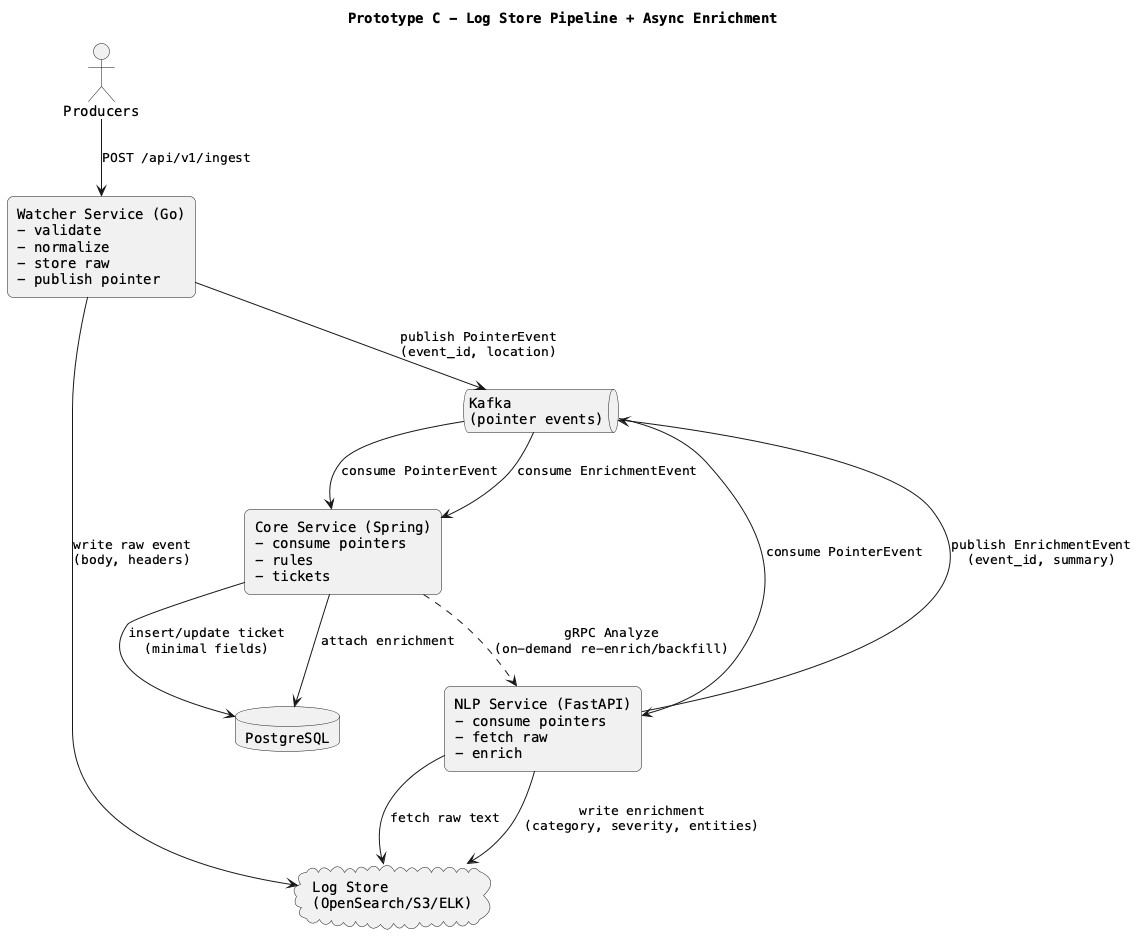
\includegraphics[width=\linewidth]{prototype-c-pipeline-async-enrichment.png}
  \caption{Prototype C: Log store pipeline with async enrichment}
\end{figure}

\subsection{Status}
Trade-offs are captured in \texttt{sections/tradeoffs.tex}. The selected target is documented in the architecture document.

\section{Trade-off Analysis (Prototype Comparison)}

This section compares the prototypes on operational complexity, performance, reliability, and developer velocity.
It does \emph{not} pick a winner yet; it defines how we will decide.

\subsection{Evaluation Criteria}
\begin{itemize}
  \item \textbf{Simplicity:} how many moving parts must be deployed and understood.
  \item \textbf{Coupling:} how strongly services depend on each other's uptime and latency.
  \item \textbf{Backpressure handling:} behavior during bursts and downstream slowdowns.
  \item \textbf{Latency:} time-to-ticket and time-to-enrichment.
  \item \textbf{Reliability:} replayability, safe retries, and failure isolation.
  \item \textbf{Operability:} debugging, observability, and day-2 operations.
  \item \textbf{Cost:} infrastructure + operational overhead.
  \item \textbf{Data retention:} raw event storage, reprocessing, and auditing.
\end{itemize}

\subsection{Comparison Summary}

\begin{longtable}{@{}p{0.18\linewidth}p{0.26\linewidth}p{0.26\linewidth}p{0.26\linewidth}@{}}
\toprule
\textbf{Dimension} & \textbf{Prototype A (Direct REST)} & \textbf{Prototype B (Broker)} & \textbf{Prototype C (Log Store + Broker)} \\
\midrule
Infra components & Lowest (3 services + DB) & Medium (adds broker + DLQ) & Highest (adds broker + log store) \\
Coupling & High (sync dependencies) & Medium (async ingestion; optional sync NLP) & Low/Medium (async by default) \\
Burst handling & Weak unless watcher buffers & Strong (broker absorbs spikes) & Strong (broker + raw storage separation) \\
Time-to-ticket & Low (direct call path) & Medium/Low (consume lag under load) & Medium/Low (consume lag; pointer events) \\
Time-to-enrichment & Low if NLP stable & Medium (async option) & Medium (async default; fetch from store) \\
Replay/reprocess & Hard (needs custom logs) & Good (replay from broker) & Best (replay pointers + reread raw) \\
Payload size limits & Tight (HTTP/request size) & Medium (broker limits) & Best (broker carries pointers only) \\
Debugging & Simple trace path & Needs queue tooling & Needs queue + store tooling \\
Cost & Lowest & Medium & Highest \\
\bottomrule
\end{longtable}

\subsection{Common Failure Modes and Mitigations}
\textbf{Applies to all prototypes:}
\begin{itemize}
  \item \textbf{Duplicate events:} use \texttt{event\_id} for idempotency and deduplication.
  \item \textbf{Hot sources:} add per-source rate limiting and sampling policies.
  \item \textbf{Noisy events:} implement suppression windows and grouping keys (e.g., \texttt{source + category + signature}).
\end{itemize}

\textbf{Prototype A specific:}
\begin{itemize}
  \item \textbf{Downstream slowness cascades:} watcher and core must enforce timeouts and fail fast.
  \item \textbf{NLP outage blocks requests:} create tickets without enrichment and enrich later via retry queue.
\end{itemize}

\textbf{Prototype B specific:}
\begin{itemize}
  \item \textbf{Poison messages:} route to DLQ after bounded retries; build replay tooling.
  \item \textbf{Exactly-once assumptions:} assume at-least-once; make consumers idempotent.
\end{itemize}

\textbf{Prototype C specific:}
\begin{itemize}
  \item \textbf{Pointer refers to missing raw payload:} enforce write-before-publish and include \texttt{content\_hash}.
  \item \textbf{Store growth:} define retention policies and index lifecycle management early.
\end{itemize}

\subsection{Decision Rubric (How We Will Choose)}
We pick the prototype that best fits the first target environment and workload.
Use these questions as the selection checklist:
\begin{enumerate}
  \item What is the peak ingestion rate and expected burst size?
  \item Is ``ticket created within X seconds'' a hard SLO?
  \item Is enrichment required for correctness, or can it be eventually consistent?
  \item Do we need replay/reprocessing for audits or model improvements?
  \item How much infrastructure is acceptable for the MVP (Kafka, log store, Supabase)?
  \item What is the operational maturity of the team running it?
\end{enumerate}

\section{Key Flows (Sequence Diagrams)}

\subsection{Reactive log ingestion $\rightarrow$ ticket $\rightarrow$ enrichment (sync)}
\begin{figure}[h]
  \centering
  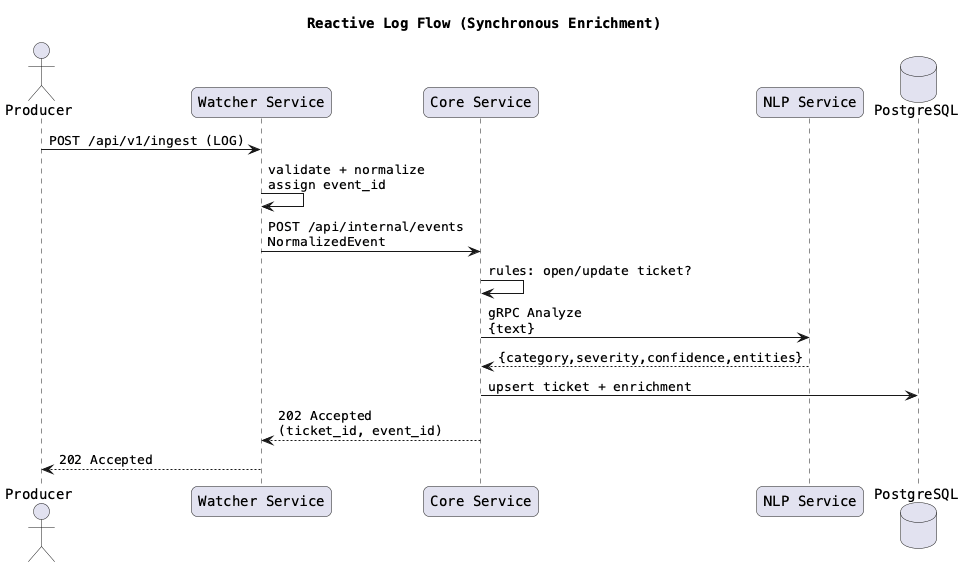
\includegraphics[width=\linewidth]{seq-reactive-sync.png}
  \caption{Synchronous enrichment flow (fits Prototype A, optional in B)}
\end{figure}

\subsection{Reactive log ingestion $\rightarrow$ async enrichment $\rightarrow$ ticket update}
\begin{figure}[h]
  \centering
  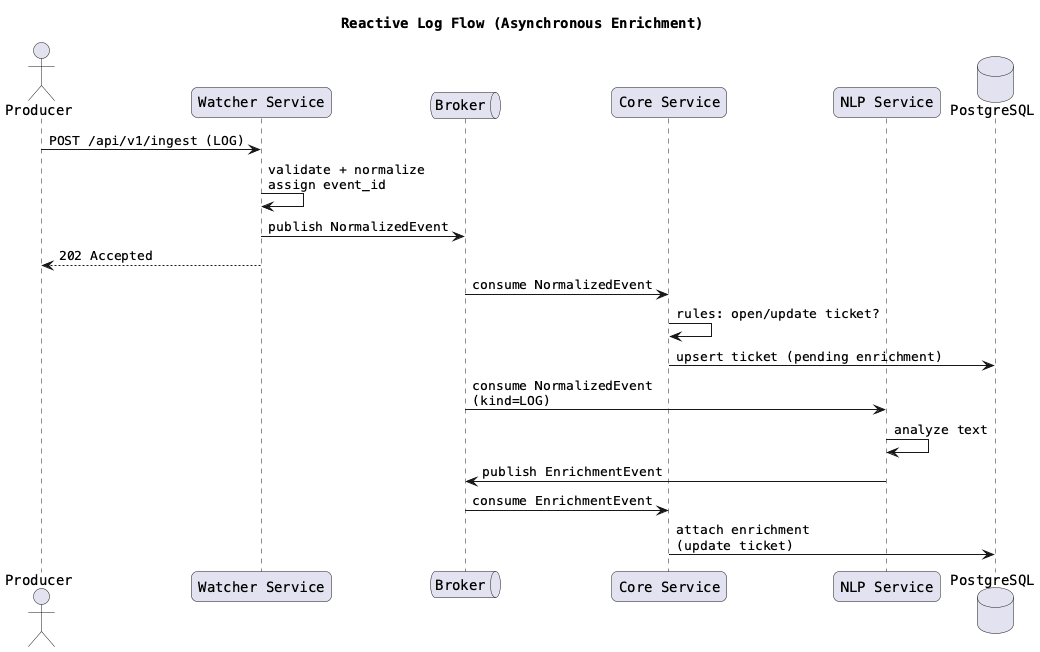
\includegraphics[width=\linewidth]{seq-reactive-async.png}
  \caption{Asynchronous enrichment flow (fits Prototype B/C)}
\end{figure}



\section{Decision: Prototype C + gRPC Internal APIs}
We proceed with \textbf{Prototype C} as the target architecture, with a critical modification:
\textbf{internal (service-to-service) APIs are gRPC}, leveraging strong Go support.

The primary runtime integration remains asynchronous (broker + pointer events), while gRPC is used for:
\begin{itemize}
  \item on-demand enrichment or re-enrichment,
  \item operational backfills and replay tooling,
  \item future internal configuration/control-plane calls.
\end{itemize}

\section{Development Environment Decisions (Local, Dockerized)}
\subsection{Message Broker: Kafka}
Kafka is the chosen broker for local development and as the default target for production.
Topics follow explicit versioning (for example, \texttt{watchdog.pointer-events.v1}).

\subsection{Database + Auth Provider: Supabase}
Supabase is the chosen provider for:
\begin{itemize}
  \item \textbf{Postgres database} (tickets, users, audit),
  \item \textbf{Auth} (JWT issuance; RBAC via claims/policies).
\end{itemize}

\textbf{Local development:} use Supabase locally (dockerized) and connect services to it.
On macOS Docker, containers reach the host via \texttt{host.docker.internal}.

\section{Open Questions}
\begin{itemize}
  \item What is the first target environment: local only, VM, or Kubernetes?
  \item Do we need multi-tenancy or a single-tenant deployment model?
  \item What are acceptable latencies for ticket creation and for enrichment to appear on tickets?
  \item What is the initial topic layout and retention policy for Kafka?
  \item What is the expected event rate (steady-state and burst)?
\end{itemize}

\end{document}
